 \documentclass{article}
\usepackage[francais]{babel}
\def\printlandscape{\special{landscape}}    
\usepackage{amsmath}
\usepackage[utf8]{inputenc}
\usepackage[T1]{fontenc} 
\usepackage{fancybox} 
\usepackage{alltt}
\usepackage{graphicx}
\usepackage{lmodern}
\usepackage[colorlinks,hyperindex,bookmarks,linkcolor=blue,citecolor=blue,urlcolor=blue]{hyperref}
\usepackage{epsf}
\usepackage{enumitem}
\usepackage{pifont}
\usepackage{hyperref}
\usepackage{authblk}
\usepackage{titling}
\usepackage{floatflt}
\usepackage{changepage}
\usepackage[margin=0.5in]{geometry}
\usepackage{parskip}
\usepackage{subfig}
\setlength{\parindent}{30pt}

\begin{document}
\begin{center}
{\huge \textbf{Rapport de Début de Projet}}
\end{center}

\begin{center}
Participants : \textit{Baudet Léo-Paul / Miniaou Lucie / Tournier Pauline / Nguyen Mathieu\\}

\end{center}
\vspace{0.05\textheight}
\begin{center}
{\LARGE \textbf{Contrôle Magnétique d'Interface Liquides}}
\end{center}

\section{Travail de Mathieu et Léo-Paul}
Léo-Paul s'est assuré dans un premier temps que les différentes méthodes de résolution numérique étaient applicables sur notre équation, notamment la méthode de Nexton. Pour cette méthode, il faut vérifier que la dérivée ne s'annule pas, peu importe le x. Une fois que cela est fait, il a pu implémenter toutes les méthodes de résolution, à savoir \textbf{la dichotomie, le point fixe de Picard et la méthode de Newton}.
\newline
Mathieu a commencé par implémenter les différents champs que l'on peut retrouver dans notre situation, plus spécialement les champs qui admettent \textbf{une invariance en y} (afin de n'avoir que x et z comme inconnues). On s'est finalement penché sur les 3 cas suivant : la nappe de courant, les deux fils à courant inversé et le dipole magnétique.
\newline
La nappe de courant est le champ le plus simple à mettre en place, car si on envoie le courant selon Oy, alors on n'a un \textbf{champ qui ne dépend que de z}. L'équation implémenté est la suivante : 

\begin{equation}
H(M) = \frac{jS}{2}\vec{u_{z}}
\label{eq01}
\end{equation}

Où j est la \textbf{densité de courant} et S est la \textbf{surface considérée dans le plan xOy}
\begin{figure}[h]
	\centering
    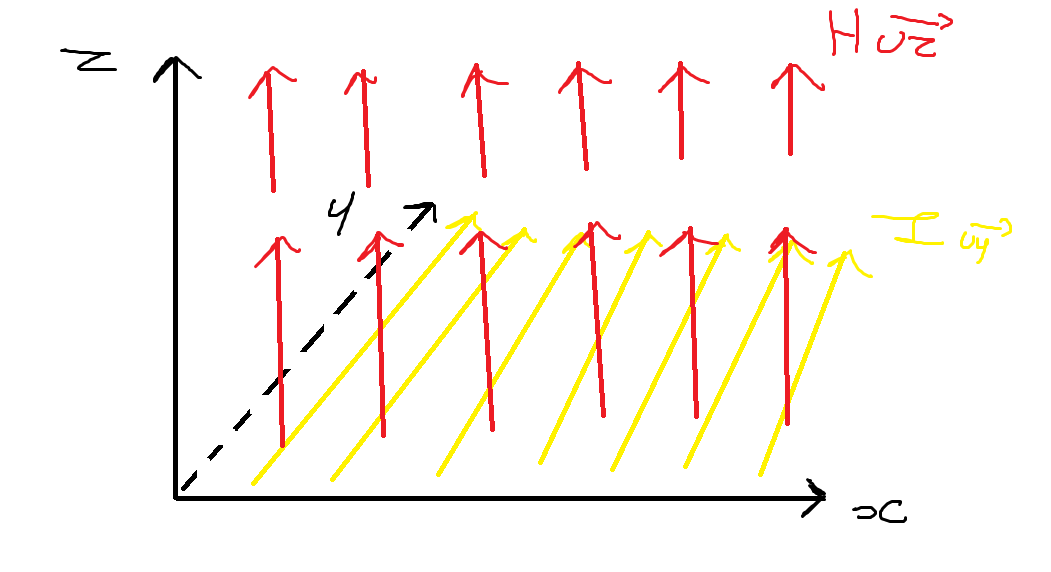
\includegraphics[width=.5\linewidth]{Nappe.png}
    
\end{figure}

Les deux fils à courant sont plus complexes à définir, car leur champ est la plupart du temps donné dans des coordonnées cylindriques, et nous voulons les implémenter en coordonnées cartésiennes. Encore une fois, on fait en sorte d'avoir une \textbf{invariance en y}. Par un théorème de Pythagore, on peut facilement déterminer la distance entre deux points à partir de \textbf{leur position en x et z}. Le point M est en $(x_{M},z_{M})$, on obtient respectivement $r_{1}$ et $r_{2}$ (respectivement la distance entre le premier fil et le point M, et la distance entre le deuxième fils et le point M) et on peut à présent utiliser la formule du \textbf{champ magnétique pour un fils de courant infini}.
\begin{equation}
r = \sqrt{(x-x_{M})^2 + (z-z_{M})^2} \indent\indent H = \frac{I}{2\pi r}
\label{eq02}
\end{equation}
On applique ces deux calculs pour obtenir les deux champs magnétiques crées par les fils 1 et 2. Pour obtenir le champ magnétique totale de ces deux fils de courant, il suffit d'additionner les deux champs crées :
\begin{equation}
H = H_{1} + H_{2}
\label{eq03}
\end{equation}
\begin{figure}[h]
	\centering
    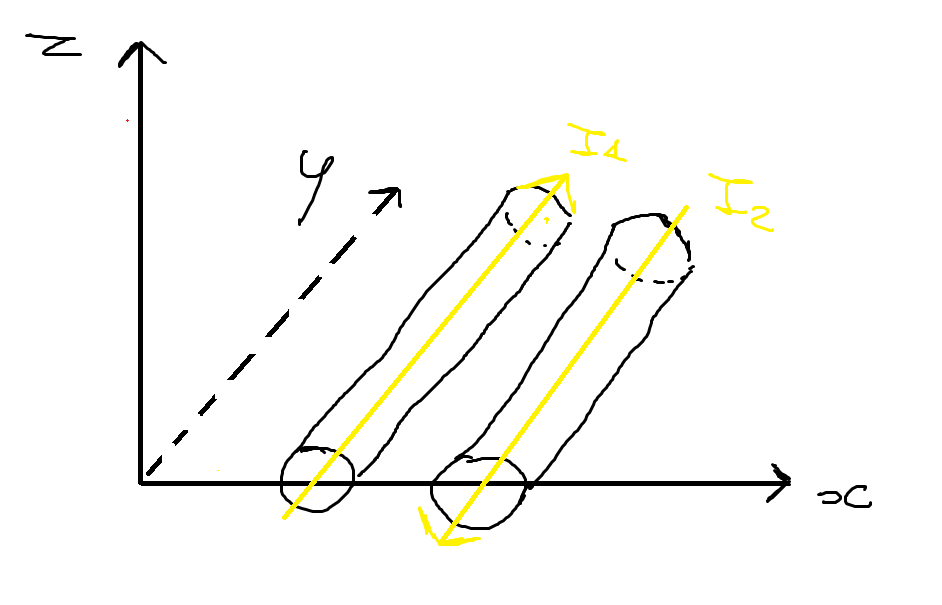
\includegraphics[width=.4\linewidth]{Fils.png}
    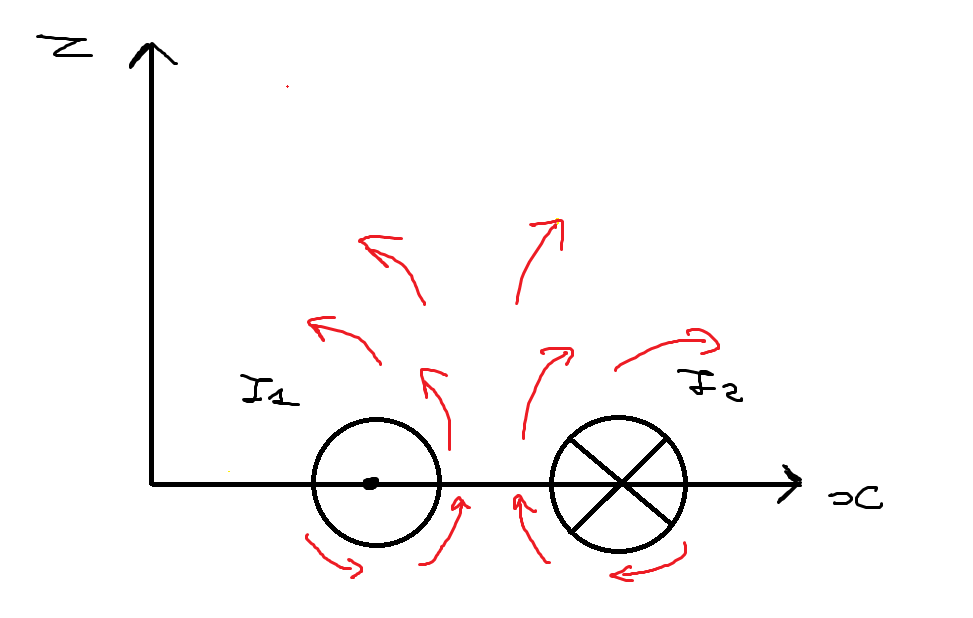
\includegraphics[width=.4\linewidth]{Fils2.png}
\end{figure}
\newpage
Pour implémenter le dipôle magnétique, j'utilise la formule en carthésien suivante en considérant le moment magnétique $m = IS$ (avec I : l'intensité et S : la surface considérée). On considère ici que cette surface est \textbf{la base du fil, indépendante de sa coordonnée en y}, les relations obtenues sont donc :
\begin{equation}
H_{x} = \frac{m}{4\pi}\frac{3zx}{r^5}\indent\indent H_{y} = \frac{m}{4\pi}\frac{3zy}{r^5}\indent\indent H_{z}=\frac{m}{4\pi}\frac{1}{r^3}[\frac{3z^2}{r^2} - 1]
\label{eq04}
\end{equation}
En rappelant que le rayon r se calcule de la manière suivante : $r = \sqrt{x^2 + y^2 +z^2}$
\begin{figure}[h]
	\centering
    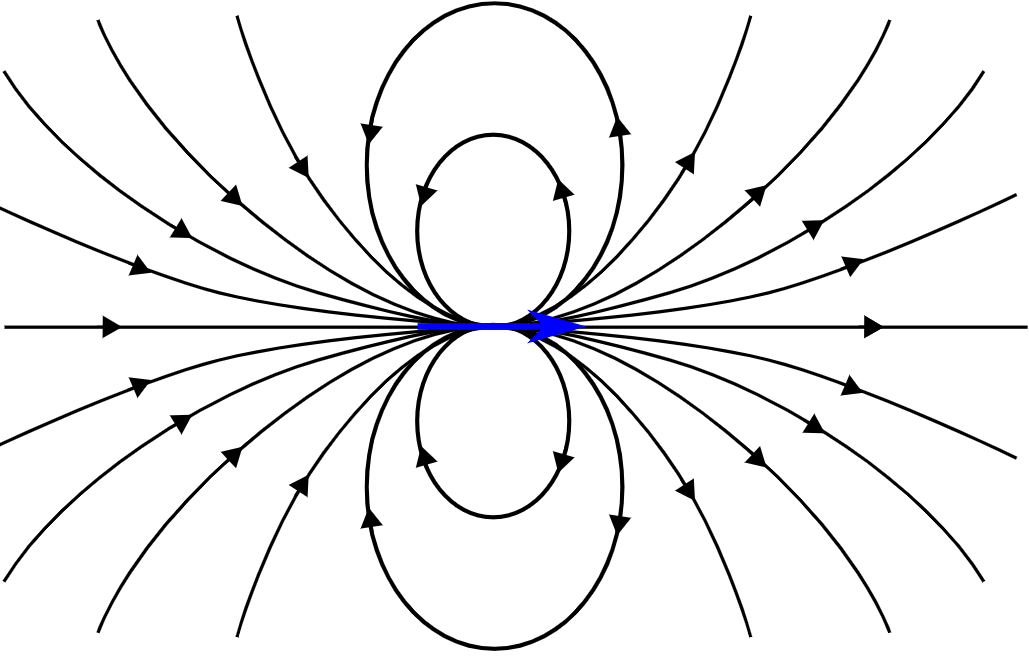
\includegraphics[width=.5\linewidth]{Dipole.png}
    
\end{figure}

Maintenant que ces champs sont mis en place, on peut à présent effectuer nos premières résolutions numériques pour déterminer la hauteur $\eta(x)$ inconnue dans notre équation $f(x,\eta(x))$ principale. Pour déterminer la fonction $\eta(x)$, on discrétise l'intervalle de x considéré en petits morceaux, et on applique notre méthode de résolution \textbf{sur chaque petit morceau}. 
\newline
Dans un premier temps, nous appliquons la \textbf{méthode de dichotomie}, qui nécessite que peu de conditions pour être appliquée. On considère un premier point $\eta_{0}$ tel que $f(\eta_{0})$ < 0 et un second point $\eta_{1} < 0$ tel que $f(\eta_{1})$ > 0. Puis on applique la dichotomie suivante : \newline 
\[
\left \{
\begin{array}{c @{=} c}
    \eta_{n} & \frac{\eta_{0} + \eta_{1}}{2} \\
    \eta_{1} & \eta_{n} \indent si \indent f(\eta_{n})  > 0 \\
    \eta_{0} & \eta_{n} \indent si \indent f(\eta_{n}) < 0
\end{array}
\right.
\]

Nous avons ensuite appliqué la méthode de Newton afin d'effectuer les résolutions numériques à chaque x discrétisé, en déterminant la hauteur $f(\eta_{x_{i}},x_{i}) = 0$. Pour cela on a appliqué l'algorithme suivant tant que $|f(\eta_n{{x_{i}}},x_{i})| > 10^{-6}$ :
\newline 
\[
\left \{
\begin{array}{c @{=} c}
    \eta_{0} & 1  \\
    \eta_{n+1} & \eta_{n} - \frac{f(\eta_{n},x_{i})}{f\prime(\eta_{n},x_{i})}
\end{array}
\right.
\]
Afin d'éviter de calculer une dérivée pour toutes les fonctions différentes (qu'on obtiendra avec tous les champs différents), nous l'avons déterminé à l'aide de la \textbf{définition de la dérivation} :

\begin{equation}
f\prime(x) = \frac{f(x + h) - f(x)}{h}
\label{eq05}
\end{equation}

Lorsqu'on l'applique sur le champ magnétique causé par \textbf{deux fils à courant inverse}, on obtient le graphique suivant :
\begin{figure}[h]
	\centering
    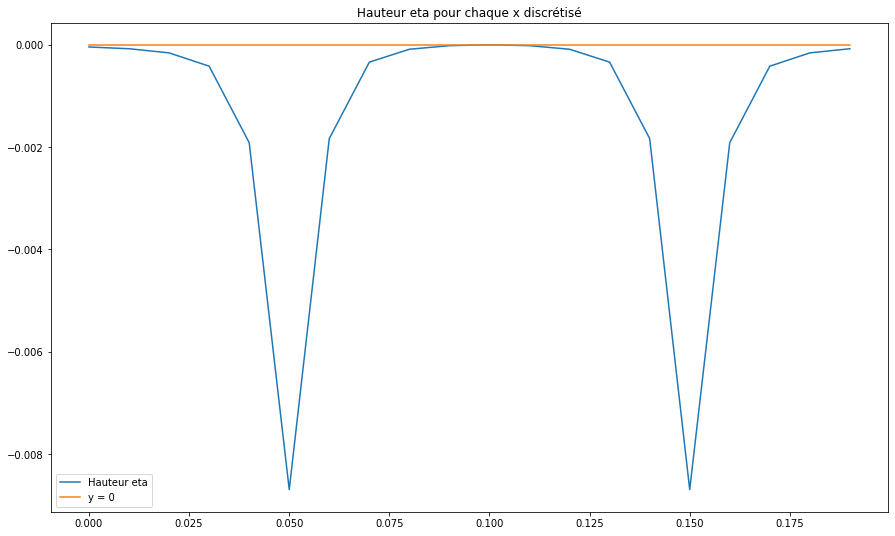
\includegraphics[width=.5\linewidth]{Hauteur.png}
    
\end{figure}

\underline{Brouillon : Spéculations et points à revoir}
Les deux pics sont dûs au fait que les deux fils se trouvent justement aux abscisses x = 0.05 et x = 0.015, et sur ces valeurs, le champ calculé à l'aide de l'équation \eqref{eq02} tend vers l'infini. Pour remédier à cela, lorsque le champ obtenu est très au dessus de l'ordre de grandeur que l'on devrait avoir, j'ai remplacé la formule utilisée par \textbf{la formule du champ magnétique pour une spire}, étant donné qu'on est la à l'intérieur d'un fil infini. Nous avons donc implémenté la formule suivante dans ces cas limites : 
\begin{equation}
H = \frac{I}{2\pi R}
\label{eq06}
\end{equation}
Avec R le \underline{rayon du fil}.
\newline
Cependant, les variations sont très faibles, de l'ordre de $10^{-5}$, ce qui n'est pas visible à l'oeil nu, donc nous pensons qu'il y a un problème, soit dans le calcul de la fonction, soit dans le calcul du champ.
\newline
Pour déterminer si le champ est correct, nous nous sommes documentés sur l'ordre de grandeur du \textbf{champ magnétique crée par un fil rectiligne infini}. D'après nos recherches, il crée un champ magnétique de l'ordre de $ B = 10^{4}$ Tesla, ou bien de l'ordre de $H = 250$ A/m.
\newline
Nous avons donc tracé le graphe du champ magnétique que l'on obtient au point $(\eta_{x_{i}},x_{i})$, avec $\eta_{x_{i}}$ le point qui annule la fonction $f(\eta_{x_{i}},x_{i}) = 0$. Nous avons alors le graphe suivant :
\begin{figure}[h]
	\centering
    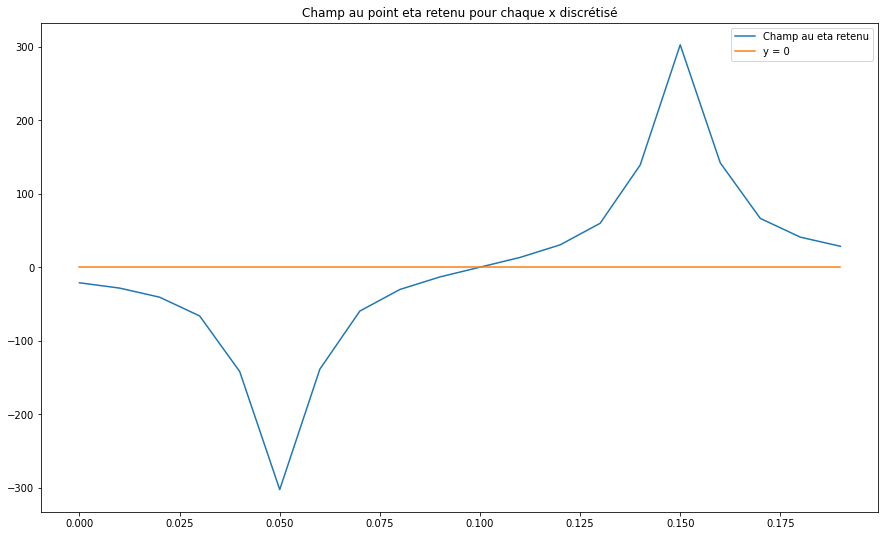
\includegraphics[width=.5\linewidth]{Champ.png}
    
\end{figure}
Les valeurs prises par le champ sont comprises entre [-300;300], nous avons donc conclut que \textbf{le problème ne provient pas du champ}.
\newline\newline
Nous avons donc essayé de déterminer l'ordre de grandeur de la fonction f(x,$\eta$), en donnant des ordres de grandeurs pour chaque terme de l'équation :
\newline
On rappelle la formule utilisée : 
\begin{equation}
(\rho_{1} - \rho_{2})g\eta + \frac{1}{2}(\chi_{1} - \chi_{2})H^{2}(x,\eta)=0
\label{eq07}
\end{equation}
En considérant que l'élément 1 est \textbf{l'air} et l'élément 2 \textbf{du chlorure de fer $FeCl_{3}$}, on a $\rho_{air}$ = 1292, $\chi_{air}$ = 0.38*10$^{-6}$, $\rho_{FeCl_{3}}$ = 2900, $\chi_{air}$ = 3000*10$^{-6}$ on pose alors : \\
$\Delta\rho$ = 10$^{-3}$, $\Delta\chi$ = $10^{-3}$, g = 10, H = $10^{-2}$ (on est toujours dans le cas du fil infini). \\
En remplaçant dans l'équation, on retrouve que $\eta$ est de l'ordre de $10^{-5}$, ce qui est effectivement ce qu'on retrouve parmi les résultats renvoyés par l'algorithme, donc on pense que le problème est dans notre expression de la fonction.
\newline\newline
Un autre problème est que la hauteur $\eta$ est toujours négative, alors que notre hauteur devrait toujours être positive ou nulle. Un simple ajout de signe négatif pourrait régler le problème mais nous n'arrivons pas savoir comment le justifier. 
\end{document}
   